\documentclass[1p]{elsarticle_modified}
%\bibliographystyle{elsarticle-num}

%\usepackage[colorlinks]{hyperref}
%\usepackage{abbrmath_seonhwa} %\Abb, \Ascr, \Acal ,\Abf, \Afrak
\usepackage{amsfonts}
\usepackage{amssymb}
\usepackage{amsmath}
\usepackage{amsthm}
\usepackage{scalefnt}
\usepackage{amsbsy}
\usepackage{kotex}
\usepackage{caption}
\usepackage{subfig}
\usepackage{color}
\usepackage{graphicx}
\usepackage{xcolor} %% white, black, red, green, blue, cyan, magenta, yellow
\usepackage{float}
\usepackage{setspace}
\usepackage{hyperref}

\usepackage{tikz}
\usetikzlibrary{arrows}

\usepackage{multirow}
\usepackage{array} % fixed length table
\usepackage{hhline}

%%%%%%%%%%%%%%%%%%%%%
\makeatletter
\renewcommand*\env@matrix[1][\arraystretch]{%
	\edef\arraystretch{#1}%
	\hskip -\arraycolsep
	\let\@ifnextchar\new@ifnextchar
	\array{*\c@MaxMatrixCols c}}
\makeatother %https://tex.stackexchange.com/questions/14071/how-can-i-increase-the-line-spacing-in-a-matrix
%%%%%%%%%%%%%%%

\usepackage[normalem]{ulem}

\newcommand{\msout}[1]{\ifmmode\text{\sout{\ensuremath{#1}}}\else\sout{#1}\fi}
%SOURCE: \msout is \stkout macro in https://tex.stackexchange.com/questions/20609/strikeout-in-math-mode

\newcommand{\cancel}[1]{
	\ifmmode
	{\color{red}\msout{#1}}
	\else
	{\color{red}\sout{#1}}
	\fi
}

\newcommand{\add}[1]{
	{\color{blue}\uwave{#1}}
}

\newcommand{\replace}[2]{
	\ifmmode
	{\color{red}\msout{#1}}{\color{blue}\uwave{#2}}
	\else
	{\color{red}\sout{#1}}{\color{blue}\uwave{#2}}
	\fi
}

\newcommand{\Sol}{\mathcal{S}} %segment
\newcommand{\D}{D} %diagram
\newcommand{\A}{\mathcal{A}} %arc


%%%%%%%%%%%%%%%%%%%%%%%%%%%%%5 test

\def\sl{\operatorname{\textup{SL}}(2,\Cbb)}
\def\psl{\operatorname{\textup{PSL}}(2,\Cbb)}
\def\quan{\mkern 1mu \triangleright \mkern 1mu}

\theoremstyle{definition}
\newtheorem{thm}{Theorem}[section]
\newtheorem{prop}[thm]{Proposition}
\newtheorem{lem}[thm]{Lemma}
\newtheorem{ques}[thm]{Question}
\newtheorem{cor}[thm]{Corollary}
\newtheorem{defn}[thm]{Definition}
\newtheorem{exam}[thm]{Example}
\newtheorem{rmk}[thm]{Remark}
\newtheorem{alg}[thm]{Algorithm}

\newcommand{\I}{\sqrt{-1}}
\begin{document}

%\begin{frontmatter}
%
%\title{Boundary parabolic representations of knots up to 8 crossings}
%
%%% Group authors per affiliation:
%\author{Yunhi Cho} 
%\address{Department of Mathematics, University of Seoul, Seoul, Korea}
%\ead{yhcho@uos.ac.kr}
%
%
%\author{Seonhwa Kim} %\fnref{s_kim}}
%\address{Center for Geometry and Physics, Institute for Basic Science, Pohang, 37673, Korea}
%\ead{ryeona17@ibs.re.kr}
%
%\author{Hyuk Kim}
%\address{Department of Mathematical Sciences, Seoul National University, Seoul 08826, Korea}
%\ead{hyukkim@snu.ac.kr}
%
%\author{Seokbeom Yoon}
%\address{Department of Mathematical Sciences, Seoul National University, Seoul, 08826,  Korea}
%\ead{sbyoon15@snu.ac.kr}
%
%\begin{abstract}
%We find all boundary parabolic representation of knots up to 8 crossings.
%
%\end{abstract}
%\begin{keyword}
%    \MSC[2010] 57M25 
%\end{keyword}
%
%\end{frontmatter}

%\linenumbers
%\tableofcontents
%
\newcommand\colored[1]{\textcolor{white}{\rule[-0.35ex]{0.8em}{1.4ex}}\kern-0.8em\color{red} #1}%
%\newcommand\colored[1]{\textcolor{white}{ #1}\kern-2.17ex	\textcolor{white}{ #1}\kern-1.81ex	\textcolor{white}{ #1}\kern-2.15ex\color{red}#1	}

{\Large $\underline{12n_{0525}~(K12n_{0525})}$}

\setlength{\tabcolsep}{10pt}
\renewcommand{\arraystretch}{1.6}
\vspace{1cm}\begin{tabular}{m{100pt}>{\centering\arraybackslash}m{274pt}}
\multirow{5}{120pt}{
	\centering
	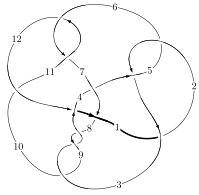
\includegraphics[width=112pt]{../../../GIT/diagram.site/Diagrams/png/2614_12n_0525.png}\\
\ \ \ A knot diagram\footnotemark}&
\allowdisplaybreaks
\textbf{Linearized knot diagam} \\
\cline{2-2}
 &
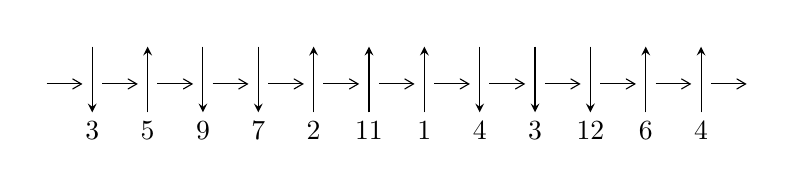
\begin{tikzpicture}[x=20pt, y=17pt]
	% nodes
	\node (C0) at (0, 0) {};
	\node (C1) at (1, 0) {};
	\node (C1U) at (1, +1) {};
	\node (C1D) at (1, -1) {3};

	\node (C2) at (2, 0) {};
	\node (C2U) at (2, +1) {};
	\node (C2D) at (2, -1) {5};

	\node (C3) at (3, 0) {};
	\node (C3U) at (3, +1) {};
	\node (C3D) at (3, -1) {9};

	\node (C4) at (4, 0) {};
	\node (C4U) at (4, +1) {};
	\node (C4D) at (4, -1) {7};

	\node (C5) at (5, 0) {};
	\node (C5U) at (5, +1) {};
	\node (C5D) at (5, -1) {2};

	\node (C6) at (6, 0) {};
	\node (C6U) at (6, +1) {};
	\node (C6D) at (6, -1) {11};

	\node (C7) at (7, 0) {};
	\node (C7U) at (7, +1) {};
	\node (C7D) at (7, -1) {1};

	\node (C8) at (8, 0) {};
	\node (C8U) at (8, +1) {};
	\node (C8D) at (8, -1) {4};

	\node (C9) at (9, 0) {};
	\node (C9U) at (9, +1) {};
	\node (C9D) at (9, -1) {3};

	\node (C10) at (10, 0) {};
	\node (C10U) at (10, +1) {};
	\node (C10D) at (10, -1) {12};

	\node (C11) at (11, 0) {};
	\node (C11U) at (11, +1) {};
	\node (C11D) at (11, -1) {6};

	\node (C12) at (12, 0) {};
	\node (C12U) at (12, +1) {};
	\node (C12D) at (12, -1) {4};
	\node (C13) at (13, 0) {};

	% arrows
	\draw[->,>={angle 60}]
	(C0) edge (C1) (C1) edge (C2) (C2) edge (C3) (C3) edge (C4) (C4) edge (C5) (C5) edge (C6) (C6) edge (C7) (C7) edge (C8) (C8) edge (C9) (C9) edge (C10) (C10) edge (C11) (C11) edge (C12) (C12) edge (C13) ;	\draw[->,>=stealth]
	(C1U) edge (C1D) (C2D) edge (C2U) (C3U) edge (C3D) (C4U) edge (C4D) (C5D) edge (C5U) (C6D) edge (C6U) (C7D) edge (C7U) (C8U) edge (C8D) (C9U) edge (C9D) (C10U) edge (C10D) (C11D) edge (C11U) (C12D) edge (C12U) ;
	\end{tikzpicture} \\
\hhline{~~} \\& 
\textbf{Solving Sequence} \\ \cline{2-2} 
 &
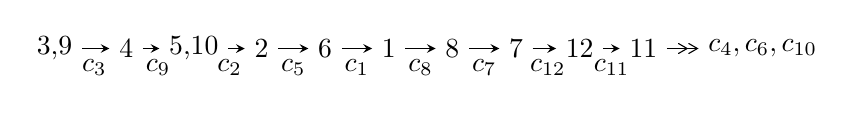
\begin{tikzpicture}[x=23pt, y=7pt]
	% node
	\node (A0) at (-1/8, 0) {3,9};
	\node (A1) at (1, 0) {4};
	\node (A2) at (33/16, 0) {5,10};
	\node (A3) at (25/8, 0) {2};
	\node (A4) at (33/8, 0) {6};
	\node (A5) at (41/8, 0) {1};
	\node (A6) at (49/8, 0) {8};
	\node (A7) at (57/8, 0) {7};
	\node (A8) at (65/8, 0) {12};
	\node (A9) at (73/8, 0) {11};
	\node (C1) at (1/2, -1) {$c_{3}$};
	\node (C2) at (3/2, -1) {$c_{9}$};
	\node (C3) at (21/8, -1) {$c_{2}$};
	\node (C4) at (29/8, -1) {$c_{5}$};
	\node (C5) at (37/8, -1) {$c_{1}$};
	\node (C6) at (45/8, -1) {$c_{8}$};
	\node (C7) at (53/8, -1) {$c_{7}$};
	\node (C8) at (61/8, -1) {$c_{12}$};
	\node (C9) at (69/8, -1) {$c_{11}$};
	\node (A10) at (11, 0) {$c_{4},c_{6},c_{10}$};

	% edge
	\draw[->,>=stealth]	
	(A0) edge (A1) (A1) edge (A2) (A2) edge (A3) (A3) edge (A4) (A4) edge (A5) (A5) edge (A6) (A6) edge (A7) (A7) edge (A8) (A8) edge (A9) ;
	\draw[->>,>={angle 60}]	
	(A9) edge (A10);
\end{tikzpicture} \\ 

\end{tabular} \\

\footnotetext{
The image of knot diagram is generated by the software ``\textbf{Draw programme}" developed by Andrew Bartholomew(\url{http://www.layer8.co.uk/maths/draw/index.htm\#Running-draw}), where we modified some parts for our purpose(\url{https://github.com/CATsTAILs/LinksPainter}).
}\phantom \\ \newline 
\centering \textbf{Ideals for irreducible components\footnotemark of $X_{\text{par}}$} 
 
\begin{align*}
I^u_{1}&=\langle 
730697 u^{21}+8724191 u^{20}+\cdots+1495432 b+38274232,\\
\phantom{I^u_{1}}&\phantom{= \langle  }-1973739 u^{21}-26703501 u^{20}+\cdots+5981728 a-159009976,\;u^{22}+11 u^{21}+\cdots+232 u+32\rangle \\
I^u_{2}&=\langle 
-10 u^{29}+31 u^{28}+\cdots+8 b-6,\;-54 u^{29} a+37 u^{29}+\cdots+104 a-100,\;u^{30}-5 u^{29}+\cdots-2 u+1\rangle \\
I^u_{3}&=\langle 
u^{11}+2 u^{10}+7 u^9+10 u^8+18 u^7+15 u^6+19 u^5+5 u^4+7 u^3-2 u^2+b+2 u,\\
\phantom{I^u_{3}}&\phantom{= \langle  }- u^{11}- u^{10}-5 u^9-3 u^8-8 u^7+3 u^6-4 u^5+14 u^4-2 u^3+8 u^2+a-4 u+1,\\
\phantom{I^u_{3}}&\phantom{= \langle  }u^{12}+2 u^{11}+7 u^{10}+10 u^9+19 u^8+17 u^7+24 u^6+11 u^5+15 u^4+2 u^3+6 u^2+1\rangle \\
I^u_{4}&=\langle 
- u^2 a+u^3- u^2+b+u,\;u^5 a-2 u^4 a-4 u^5+5 u^3 a+5 u^4-6 u^2 a-11 u^3+a^2+5 a u+9 u^2-2 a-10 u,\\
\phantom{I^u_{4}}&\phantom{= \langle  }u^6- u^5+3 u^4-2 u^3+3 u^2+1\rangle \\
\\
\end{align*}
\raggedright * 4 irreducible components of $\dim_{\mathbb{C}}=0$, with total 106 representations.\\
\footnotetext{All coefficients of polynomials are rational numbers. But the coefficients are sometimes approximated in decimal forms when there is not enough margin.}
\newpage
\renewcommand{\arraystretch}{1}
\centering \section*{I. $I^u_{1}= \langle 7.31\times10^{5} u^{21}+8.72\times10^{6} u^{20}+\cdots+1.50\times10^{6} b+3.83\times10^{7},\;-1.97\times10^{6} u^{21}-2.67\times10^{7} u^{20}+\cdots+5.98\times10^{6} a-1.59\times10^{8},\;u^{22}+11 u^{21}+\cdots+232 u+32 \rangle$}
\flushleft \textbf{(i) Arc colorings}\\
\begin{tabular}{m{7pt} m{180pt} m{7pt} m{180pt} }
\flushright $a_{3}=$&$\begin{pmatrix}1\\0\end{pmatrix}$ \\
\flushright $a_{9}=$&$\begin{pmatrix}0\\u\end{pmatrix}$ \\
\flushright $a_{4}=$&$\begin{pmatrix}1\\u^2\end{pmatrix}$ \\
\flushright $a_{5}=$&$\begin{pmatrix}0.329961 u^{21}+4.46418 u^{20}+\cdots+167.160 u+26.5826\\-0.488619 u^{21}-5.83389 u^{20}+\cdots-164.041 u-25.5941\end{pmatrix}$ \\
\flushright $a_{10}=$&$\begin{pmatrix}- u\\u\end{pmatrix}$ \\
\flushright $a_{2}=$&$\begin{pmatrix}-0.678659 u^{21}-6.54536 u^{20}+\cdots-66.3494 u-8.74650\\0.549186 u^{21}+5.23031 u^{20}+\cdots+73.2841 u+11.2249\end{pmatrix}$ \\
\flushright $a_{6}=$&$\begin{pmatrix}-0.309352 u^{21}-2.39786 u^{20}+\cdots+59.0207 u+10.7541\\-0.730680 u^{21}-8.31181 u^{20}+\cdots-218.761 u-33.2810\end{pmatrix}$ \\
\flushright $a_{1}=$&$\begin{pmatrix}-0.129473 u^{21}-1.31505 u^{20}+\cdots+6.93466 u+2.47838\\0.549186 u^{21}+5.23031 u^{20}+\cdots+73.2841 u+11.2249\end{pmatrix}$ \\
\flushright $a_{8}=$&$\begin{pmatrix}u\\u^3+u\end{pmatrix}$ \\
\flushright $a_{7}=$&$\begin{pmatrix}0.770630 u^{21}+8.00468 u^{20}+\cdots+111.293 u+15.5266\\0.580458 u^{21}+6.16373 u^{20}+\cdots+148.964 u+22.7178\end{pmatrix}$ \\
\flushright $a_{12}=$&$\begin{pmatrix}-0.459930 u^{21}-4.72878 u^{20}+\cdots-87.5298 u-12.2394\\0.109153 u^{21}+1.41941 u^{20}+\cdots+32.5161 u+4.14313\end{pmatrix}$ \\
\flushright $a_{11}=$&$\begin{pmatrix}-0.709930 u^{21}-7.22878 u^{20}+\cdots-117.030 u-16.7394\\0.359153 u^{21}+3.66941 u^{20}+\cdots+37.0161 u+4.14313\end{pmatrix}$\\&\end{tabular}
\flushleft \textbf{(ii) Obstruction class $= -1$}\\~\\
\flushleft \textbf{(iii) Cusp Shapes $= -\frac{297700}{186929} u^{21}-\frac{2758587}{186929} u^{20}+\cdots-\frac{6073132}{186929} u-\frac{1067206}{186929}$}\\~\\
\newpage\renewcommand{\arraystretch}{1}
\flushleft \textbf{(iv) u-Polynomials at the component}\newline \\
\begin{tabular}{m{50pt}|m{274pt}}
Crossings & \hspace{64pt}u-Polynomials at each crossing \\
\hline $$\begin{aligned}c_{1},c_{10}\end{aligned}$$&$\begin{aligned}
&u^{22}+13 u^{21}+\cdots+6 u+1
\end{aligned}$\\
\hline $$\begin{aligned}c_{2},c_{5},c_{6}\\c_{11}\end{aligned}$$&$\begin{aligned}
&u^{22}+u^{21}+\cdots-2 u+1
\end{aligned}$\\
\hline $$\begin{aligned}c_{3},c_{8},c_{9}\end{aligned}$$&$\begin{aligned}
&u^{22}+11 u^{21}+\cdots+232 u+32
\end{aligned}$\\
\hline $$\begin{aligned}c_{4}\end{aligned}$$&$\begin{aligned}
&u^{22}-15 u^{21}+\cdots-480 u+64
\end{aligned}$\\
\hline $$\begin{aligned}c_{7},c_{12}\end{aligned}$$&$\begin{aligned}
&u^{22}+13 u^{20}+\cdots- u+1
\end{aligned}$\\
\hline
\end{tabular}\\~\\
\newpage\renewcommand{\arraystretch}{1}
\flushleft \textbf{(v) Riley Polynomials at the component}\newline \\
\begin{tabular}{m{50pt}|m{274pt}}
Crossings & \hspace{64pt}Riley Polynomials at each crossing \\
\hline $$\begin{aligned}c_{1},c_{10}\end{aligned}$$&$\begin{aligned}
&y^{22}+y^{21}+\cdots+34 y+1
\end{aligned}$\\
\hline $$\begin{aligned}c_{2},c_{5},c_{6}\\c_{11}\end{aligned}$$&$\begin{aligned}
&y^{22}+13 y^{21}+\cdots+6 y+1
\end{aligned}$\\
\hline $$\begin{aligned}c_{3},c_{8},c_{9}\end{aligned}$$&$\begin{aligned}
&y^{22}+11 y^{21}+\cdots+3264 y+1024
\end{aligned}$\\
\hline $$\begin{aligned}c_{4}\end{aligned}$$&$\begin{aligned}
&y^{22}+7 y^{21}+\cdots+39936 y+4096
\end{aligned}$\\
\hline $$\begin{aligned}c_{7},c_{12}\end{aligned}$$&$\begin{aligned}
&y^{22}+26 y^{21}+\cdots+17 y+1
\end{aligned}$\\
\hline
\end{tabular}\\~\\
\newpage\flushleft \textbf{(vi) Complex Volumes and Cusp Shapes}
$$\begin{array}{c|c|c}  
\text{Solutions to }I^u_{1}& \I (\text{vol} + \sqrt{-1}CS) & \text{Cusp shape}\\
 \hline 
\begin{aligned}
u &= -0.767910 + 0.699836 I \\
a &= \phantom{-}0.888145 - 0.307129 I \\
b &= -0.688888 - 0.277789 I\end{aligned}
 & -0.286662 + 0.737446 I & \phantom{-}3.26178 - 2.36364 I \\ \hline\begin{aligned}
u &= -0.767910 - 0.699836 I \\
a &= \phantom{-}0.888145 + 0.307129 I \\
b &= -0.688888 + 0.277789 I\end{aligned}
 & -0.286662 - 0.737446 I & \phantom{-}3.26178 + 2.36364 I \\ \hline\begin{aligned}
u &= -0.350255 + 1.075900 I \\
a &= \phantom{-}0.81263 - 1.53152 I \\
b &= -0.240178 + 0.810554 I\end{aligned}
 & -2.88260 + 1.01233 I & -4.09792 + 3.96823 I \\ \hline\begin{aligned}
u &= -0.350255 - 1.075900 I \\
a &= \phantom{-}0.81263 + 1.53152 I \\
b &= -0.240178 - 0.810554 I\end{aligned}
 & -2.88260 - 1.01233 I & -4.09792 - 3.96823 I \\ \hline\begin{aligned}
u &= -1.033280 + 0.527627 I \\
a &= -0.721729 - 0.194727 I \\
b &= \phantom{-}0.417851 - 1.163520 I\end{aligned}
 & -8.25550 - 1.54810 I & -5.19018 + 2.03970 I \\ \hline\begin{aligned}
u &= -1.033280 - 0.527627 I \\
a &= -0.721729 + 0.194727 I \\
b &= \phantom{-}0.417851 + 1.163520 I\end{aligned}
 & -8.25550 + 1.54810 I & -5.19018 - 2.03970 I \\ \hline\begin{aligned}
u &= \phantom{-}0.755708 + 0.364616 I \\
a &= \phantom{-}0.685218 + 0.575896 I \\
b &= -0.063685 + 1.154200 I\end{aligned}
 & -4.85462 - 1.77876 I & -4.79807 + 3.91708 I \\ \hline\begin{aligned}
u &= \phantom{-}0.755708 - 0.364616 I \\
a &= \phantom{-}0.685218 - 0.575896 I \\
b &= -0.063685 - 1.154200 I\end{aligned}
 & -4.85462 + 1.77876 I & -4.79807 - 3.91708 I \\ \hline\begin{aligned}
u &= -0.774895 + 1.020220 I \\
a &= -0.766277 + 0.769605 I \\
b &= \phantom{-}0.885411 - 0.402143 I\end{aligned}
 & \phantom{-}0.61034 + 5.16314 I & \phantom{-}3.96974 - 2.90756 I \\ \hline\begin{aligned}
u &= -0.774895 - 1.020220 I \\
a &= -0.766277 - 0.769605 I \\
b &= \phantom{-}0.885411 + 0.402143 I\end{aligned}
 & \phantom{-}0.61034 - 5.16314 I & \phantom{-}3.96974 + 2.90756 I\\
 \hline 
 \end{array}$$\newpage$$\begin{array}{c|c|c}  
\text{Solutions to }I^u_{1}& \I (\text{vol} + \sqrt{-1}CS) & \text{Cusp shape}\\
 \hline 
\begin{aligned}
u &= -1.221500 + 0.677927 I \\
a &= \phantom{-}0.567702 - 0.117730 I \\
b &= -0.558982 + 1.253320 I\end{aligned}
 & -6.12965 - 9.37239 I & -3.35170 + 5.78555 I \\ \hline\begin{aligned}
u &= -1.221500 - 0.677927 I \\
a &= \phantom{-}0.567702 + 0.117730 I \\
b &= -0.558982 - 1.253320 I\end{aligned}
 & -6.12965 + 9.37239 I & -3.35170 - 5.78555 I \\ \hline\begin{aligned}
u &= -0.127935 + 1.398640 I \\
a &= -1.71401 - 0.32772 I \\
b &= \phantom{-}0.565971 + 0.644936 I\end{aligned}
 & \phantom{-}6.04024 + 2.92164 I & \phantom{-}4.28614 + 0.75325 I \\ \hline\begin{aligned}
u &= -0.127935 - 1.398640 I \\
a &= -1.71401 + 0.32772 I \\
b &= \phantom{-}0.565971 - 0.644936 I\end{aligned}
 & \phantom{-}6.04024 - 2.92164 I & \phantom{-}4.28614 - 0.75325 I \\ \hline\begin{aligned}
u &= -0.304981 + 0.451421 I \\
a &= \phantom{-}0.960223 - 0.185150 I \\
b &= -0.310004 - 0.375864 I\end{aligned}
 & \phantom{-}0.090652 + 0.977959 I & \phantom{-}1.72728 - 6.82657 I \\ \hline\begin{aligned}
u &= -0.304981 - 0.451421 I \\
a &= \phantom{-}0.960223 + 0.185150 I \\
b &= -0.310004 + 0.375864 I\end{aligned}
 & \phantom{-}0.090652 - 0.977959 I & \phantom{-}1.72728 + 6.82657 I \\ \hline\begin{aligned}
u &= -0.76091 + 1.25738 I \\
a &= \phantom{-}1.92912 + 0.01305 I \\
b &= -0.557890 - 1.095380 I\end{aligned}
 & -5.97217 + 8.17735 I & -2.07600 - 6.92513 I \\ \hline\begin{aligned}
u &= -0.76091 - 1.25738 I \\
a &= \phantom{-}1.92912 - 0.01305 I \\
b &= -0.557890 + 1.095380 I\end{aligned}
 & -5.97217 - 8.17735 I & -2.07600 + 6.92513 I \\ \hline\begin{aligned}
u &= -0.89339 + 1.20903 I \\
a &= -1.79322 + 0.05043 I \\
b &= \phantom{-}0.663517 + 1.230310 I\end{aligned}
 & -4.4232 + 16.8853 I & -1.04656 - 9.40882 I \\ \hline\begin{aligned}
u &= -0.89339 - 1.20903 I \\
a &= -1.79322 - 0.05043 I \\
b &= \phantom{-}0.663517 - 1.230310 I\end{aligned}
 & -4.4232 - 16.8853 I & -1.04656 + 9.40882 I\\
 \hline 
 \end{array}$$\newpage$$\begin{array}{c|c|c}  
\text{Solutions to }I^u_{1}& \I (\text{vol} + \sqrt{-1}CS) & \text{Cusp shape}\\
 \hline 
\begin{aligned}
u &= -0.02066 + 1.63363 I \\
a &= -0.972799 + 0.791268 I \\
b &= \phantom{-}0.386878 - 1.096150 I\end{aligned}
 & \phantom{-}3.03407 - 4.86939 I & -4.68451 + 3.83035 I \\ \hline\begin{aligned}
u &= -0.02066 - 1.63363 I \\
a &= -0.972799 - 0.791268 I \\
b &= \phantom{-}0.386878 + 1.096150 I\end{aligned}
 & \phantom{-}3.03407 + 4.86939 I & -4.68451 - 3.83035 I\\
 \hline 
 \end{array}$$\newpage\newpage\renewcommand{\arraystretch}{1}
\centering \section*{II. $I^u_{2}= \langle -10 u^{29}+31 u^{28}+\cdots+8 b-6,\;-54 u^{29} a+37 u^{29}+\cdots+104 a-100,\;u^{30}-5 u^{29}+\cdots-2 u+1 \rangle$}
\flushleft \textbf{(i) Arc colorings}\\
\begin{tabular}{m{7pt} m{180pt} m{7pt} m{180pt} }
\flushright $a_{3}=$&$\begin{pmatrix}1\\0\end{pmatrix}$ \\
\flushright $a_{9}=$&$\begin{pmatrix}0\\u\end{pmatrix}$ \\
\flushright $a_{4}=$&$\begin{pmatrix}1\\u^2\end{pmatrix}$ \\
\flushright $a_{5}=$&$\begin{pmatrix}a\\\frac{5}{4} u^{29}-\frac{31}{8} u^{28}+\cdots+\frac{25}{8} u+\frac{3}{4}\end{pmatrix}$ \\
\flushright $a_{10}=$&$\begin{pmatrix}- u\\u\end{pmatrix}$ \\
\flushright $a_{2}=$&$\begin{pmatrix}-\frac{3}{2} u^{29} a+\frac{5}{4} u^{29}+\cdots-\frac{7}{8} a+\frac{3}{8}\\\frac{7}{8} u^{29} a-\frac{1}{8} u^{29}+\cdots-\frac{3}{4} a-\frac{29}{8}\end{pmatrix}$ \\
\flushright $a_{6}=$&$\begin{pmatrix}-0.500000 a u^{29}+2.12500 u^{29}+\cdots-1.62500 a-2.75000\\-\frac{3}{2} u^{29} a-\frac{11}{2} u^{29}+\cdots+2 a+\frac{69}{8}\end{pmatrix}$ \\
\flushright $a_{1}=$&$\begin{pmatrix}-\frac{5}{8} u^{29} a+\frac{9}{8} u^{29}+\cdots-\frac{13}{8} a-\frac{13}{4}\\\frac{7}{8} u^{29} a-\frac{1}{8} u^{29}+\cdots-\frac{3}{4} a-\frac{29}{8}\end{pmatrix}$ \\
\flushright $a_{8}=$&$\begin{pmatrix}u\\u^3+u\end{pmatrix}$ \\
\flushright $a_{7}=$&$\begin{pmatrix}-4 u^{29} a+4 u^{29}+\cdots+\frac{19}{4} a-\frac{19}{4}\\u^{29} a+\frac{9}{4} u^{29}+\cdots+\frac{3}{4} a-\frac{9}{8}\end{pmatrix}$ \\
\flushright $a_{12}=$&$\begin{pmatrix}-2 u^{29} a-\frac{5}{8} u^{29}+\cdots+\frac{3}{8} a+\frac{15}{8}\\\frac{5}{4} u^{29} a+\frac{13}{4} u^{29}+\cdots-\frac{5}{8} a-\frac{49}{8}\end{pmatrix}$ \\
\flushright $a_{11}=$&$\begin{pmatrix}-3 u^{29} a+\frac{15}{8} u^{29}+\cdots+\frac{11}{2} a-\frac{5}{2}\\\frac{3}{4} u^{29} a-\frac{13}{4} u^{29}+\cdots-\frac{5}{4} a-\frac{1}{8}\end{pmatrix}$\\&\end{tabular}
\flushleft \textbf{(ii) Obstruction class $= -1$}\\~\\
\flushleft \textbf{(iii) Cusp Shapes $= 19 u^{29}-\frac{169}{2} u^{28}+\cdots+26 u-\frac{5}{2}$}\\~\\
\newpage\renewcommand{\arraystretch}{1}
\flushleft \textbf{(iv) u-Polynomials at the component}\newline \\
\begin{tabular}{m{50pt}|m{274pt}}
Crossings & \hspace{64pt}u-Polynomials at each crossing \\
\hline $$\begin{aligned}c_{1},c_{10}\end{aligned}$$&$\begin{aligned}
&u^{60}+30 u^{59}+\cdots+31603 u+2209
\end{aligned}$\\
\hline $$\begin{aligned}c_{2},c_{5},c_{6}\\c_{11}\end{aligned}$$&$\begin{aligned}
&u^{60}-2 u^{59}+\cdots+81 u+47
\end{aligned}$\\
\hline $$\begin{aligned}c_{3},c_{8},c_{9}\end{aligned}$$&$\begin{aligned}
&(u^{30}-5 u^{29}+\cdots-2 u+1)^{2}
\end{aligned}$\\
\hline $$\begin{aligned}c_{4}\end{aligned}$$&$\begin{aligned}
&(u^{30}+6 u^{29}+\cdots+9 u+1)^{2}
\end{aligned}$\\
\hline $$\begin{aligned}c_{7},c_{12}\end{aligned}$$&$\begin{aligned}
&u^{60}+5 u^{59}+\cdots-18 u+1
\end{aligned}$\\
\hline
\end{tabular}\\~\\
\newpage\renewcommand{\arraystretch}{1}
\flushleft \textbf{(v) Riley Polynomials at the component}\newline \\
\begin{tabular}{m{50pt}|m{274pt}}
Crossings & \hspace{64pt}Riley Polynomials at each crossing \\
\hline $$\begin{aligned}c_{1},c_{10}\end{aligned}$$&$\begin{aligned}
&y^{60}+6 y^{59}+\cdots-90081877 y+4879681
\end{aligned}$\\
\hline $$\begin{aligned}c_{2},c_{5},c_{6}\\c_{11}\end{aligned}$$&$\begin{aligned}
&y^{60}+30 y^{59}+\cdots+31603 y+2209
\end{aligned}$\\
\hline $$\begin{aligned}c_{3},c_{8},c_{9}\end{aligned}$$&$\begin{aligned}
&(y^{30}+9 y^{29}+\cdots+14 y+1)^{2}
\end{aligned}$\\
\hline $$\begin{aligned}c_{4}\end{aligned}$$&$\begin{aligned}
&(y^{30}+10 y^{29}+\cdots-9 y+1)^{2}
\end{aligned}$\\
\hline $$\begin{aligned}c_{7},c_{12}\end{aligned}$$&$\begin{aligned}
&y^{60}+39 y^{59}+\cdots-40 y+1
\end{aligned}$\\
\hline
\end{tabular}\\~\\
\newpage\flushleft \textbf{(vi) Complex Volumes and Cusp Shapes}
$$\begin{array}{c|c|c}  
\text{Solutions to }I^u_{2}& \I (\text{vol} + \sqrt{-1}CS) & \text{Cusp shape}\\
 \hline 
\begin{aligned}
u &= -0.408738 + 0.809128 I \\
a &= \phantom{-}1.47348 + 0.03228 I \\
b &= -0.881093 - 0.652728 I\end{aligned}
 & \phantom{-}1.95297 + 0.83755 I & \phantom{-}3.80919 - 0.73546 I \\ \hline\begin{aligned}
u &= -0.408738 + 0.809128 I \\
a &= \phantom{-}0.65867 + 1.49537 I \\
b &= \phantom{-}0.483976 - 0.827208 I\end{aligned}
 & \phantom{-}1.95297 + 0.83755 I & \phantom{-}3.80919 - 0.73546 I \\ \hline\begin{aligned}
u &= -0.408738 - 0.809128 I \\
a &= \phantom{-}1.47348 - 0.03228 I \\
b &= -0.881093 + 0.652728 I\end{aligned}
 & \phantom{-}1.95297 - 0.83755 I & \phantom{-}3.80919 + 0.73546 I \\ \hline\begin{aligned}
u &= -0.408738 - 0.809128 I \\
a &= \phantom{-}0.65867 - 1.49537 I \\
b &= \phantom{-}0.483976 + 0.827208 I\end{aligned}
 & \phantom{-}1.95297 - 0.83755 I & \phantom{-}3.80919 + 0.73546 I \\ \hline\begin{aligned}
u &= \phantom{-}0.204797 + 0.865298 I \\
a &= \phantom{-}0.913167 + 0.827489 I \\
b &= -0.717809 - 1.010560 I\end{aligned}
 & \phantom{-}0.86908 + 5.05707 I & \phantom{-}0.52377 - 4.80046 I \\ \hline\begin{aligned}
u &= \phantom{-}0.204797 + 0.865298 I \\
a &= \phantom{-}0.79610 - 2.03259 I \\
b &= \phantom{-}0.378609 + 0.969447 I\end{aligned}
 & \phantom{-}0.86908 + 5.05707 I & \phantom{-}0.52377 - 4.80046 I \\ \hline\begin{aligned}
u &= \phantom{-}0.204797 - 0.865298 I \\
a &= \phantom{-}0.913167 - 0.827489 I \\
b &= -0.717809 + 1.010560 I\end{aligned}
 & \phantom{-}0.86908 - 5.05707 I & \phantom{-}0.52377 + 4.80046 I \\ \hline\begin{aligned}
u &= \phantom{-}0.204797 - 0.865298 I \\
a &= \phantom{-}0.79610 + 2.03259 I \\
b &= \phantom{-}0.378609 - 0.969447 I\end{aligned}
 & \phantom{-}0.86908 - 5.05707 I & \phantom{-}0.52377 + 4.80046 I \\ \hline\begin{aligned}
u &= \phantom{-}0.846145 + 0.766192 I \\
a &= -0.742838 + 0.117308 I \\
b &= \phantom{-}0.633812 - 0.058357 I\end{aligned}
 & -5.03543 - 2.48830 I & -2.08110 + 3.16963 I \\ \hline\begin{aligned}
u &= \phantom{-}0.846145 + 0.766192 I \\
a &= \phantom{-}0.161640 + 0.601130 I \\
b &= \phantom{-}0.123075 + 1.176780 I\end{aligned}
 & -5.03543 - 2.48830 I & -2.08110 + 3.16963 I\\
 \hline 
 \end{array}$$\newpage$$\begin{array}{c|c|c}  
\text{Solutions to }I^u_{2}& \I (\text{vol} + \sqrt{-1}CS) & \text{Cusp shape}\\
 \hline 
\begin{aligned}
u &= \phantom{-}0.846145 - 0.766192 I \\
a &= -0.742838 - 0.117308 I \\
b &= \phantom{-}0.633812 + 0.058357 I\end{aligned}
 & -5.03543 + 2.48830 I & -2.08110 - 3.16963 I \\ \hline\begin{aligned}
u &= \phantom{-}0.846145 - 0.766192 I \\
a &= \phantom{-}0.161640 - 0.601130 I \\
b &= \phantom{-}0.123075 - 1.176780 I\end{aligned}
 & -5.03543 + 2.48830 I & -2.08110 - 3.16963 I \\ \hline\begin{aligned}
u &= \phantom{-}0.476164 + 0.624124 I \\
a &= \phantom{-}1.065700 + 0.769850 I \\
b &= -0.560439 + 1.270490 I\end{aligned}
 & -0.16540 - 7.91184 I & -1.25799 + 13.37489 I \\ \hline\begin{aligned}
u &= \phantom{-}0.476164 + 0.624124 I \\
a &= -3.03202 - 0.17816 I \\
b &= \phantom{-}0.670131 - 1.010730 I\end{aligned}
 & -0.16540 - 7.91184 I & -1.25799 + 13.37489 I \\ \hline\begin{aligned}
u &= \phantom{-}0.476164 - 0.624124 I \\
a &= \phantom{-}1.065700 - 0.769850 I \\
b &= -0.560439 - 1.270490 I\end{aligned}
 & -0.16540 + 7.91184 I & -1.25799 - 13.37489 I \\ \hline\begin{aligned}
u &= \phantom{-}0.476164 - 0.624124 I \\
a &= -3.03202 + 0.17816 I \\
b &= \phantom{-}0.670131 + 1.010730 I\end{aligned}
 & -0.16540 + 7.91184 I & -1.25799 - 13.37489 I \\ \hline\begin{aligned}
u &= \phantom{-}0.843824 + 0.910765 I \\
a &= \phantom{-}0.922245 + 0.095668 I \\
b &= -0.146948 + 1.374310 I\end{aligned}
 & -5.24308 - 3.14036 I & \phantom{-}3.38309 + 6.95597 I \\ \hline\begin{aligned}
u &= \phantom{-}0.843824 + 0.910765 I \\
a &= \phantom{-}0.418535 + 0.014710 I \\
b &= \phantom{-}0.036650 + 0.609588 I\end{aligned}
 & -5.24308 - 3.14036 I & \phantom{-}3.38309 + 6.95597 I \\ \hline\begin{aligned}
u &= \phantom{-}0.843824 - 0.910765 I \\
a &= \phantom{-}0.922245 - 0.095668 I \\
b &= -0.146948 - 1.374310 I\end{aligned}
 & -5.24308 + 3.14036 I & \phantom{-}3.38309 - 6.95597 I \\ \hline\begin{aligned}
u &= \phantom{-}0.843824 - 0.910765 I \\
a &= \phantom{-}0.418535 - 0.014710 I \\
b &= \phantom{-}0.036650 - 0.609588 I\end{aligned}
 & -5.24308 + 3.14036 I & \phantom{-}3.38309 - 6.95597 I\\
 \hline 
 \end{array}$$\newpage$$\begin{array}{c|c|c}  
\text{Solutions to }I^u_{2}& \I (\text{vol} + \sqrt{-1}CS) & \text{Cusp shape}\\
 \hline 
\begin{aligned}
u &= \phantom{-}0.535931 + 0.532997 I \\
a &= \phantom{-}1.74162 - 0.15387 I \\
b &= -0.945912 + 0.839676 I\end{aligned}
 & \phantom{-}1.99448 - 4.75213 I & \phantom{-}1.25920 + 8.38226 I \\ \hline\begin{aligned}
u &= \phantom{-}0.535931 + 0.532997 I \\
a &= -1.15336 - 2.63260 I \\
b &= \phantom{-}0.461109 - 0.821998 I\end{aligned}
 & \phantom{-}1.99448 - 4.75213 I & \phantom{-}1.25920 + 8.38226 I \\ \hline\begin{aligned}
u &= \phantom{-}0.535931 - 0.532997 I \\
a &= \phantom{-}1.74162 + 0.15387 I \\
b &= -0.945912 - 0.839676 I\end{aligned}
 & \phantom{-}1.99448 + 4.75213 I & \phantom{-}1.25920 - 8.38226 I \\ \hline\begin{aligned}
u &= \phantom{-}0.535931 - 0.532997 I \\
a &= -1.15336 + 2.63260 I \\
b &= \phantom{-}0.461109 + 0.821998 I\end{aligned}
 & \phantom{-}1.99448 + 4.75213 I & \phantom{-}1.25920 - 8.38226 I \\ \hline\begin{aligned}
u &= -0.009746 + 0.748854 I \\
a &= \phantom{-}0.263930 - 0.170722 I \\
b &= -0.891285 - 0.086936 I\end{aligned}
 & \phantom{-}3.73099 + 2.66963 I & \phantom{-}10.94282 - 2.46654 I \\ \hline\begin{aligned}
u &= -0.009746 + 0.748854 I \\
a &= -2.60774 - 1.78017 I \\
b &= \phantom{-}0.695330 + 0.857378 I\end{aligned}
 & \phantom{-}3.73099 + 2.66963 I & \phantom{-}10.94282 - 2.46654 I \\ \hline\begin{aligned}
u &= -0.009746 - 0.748854 I \\
a &= \phantom{-}0.263930 + 0.170722 I \\
b &= -0.891285 + 0.086936 I\end{aligned}
 & \phantom{-}3.73099 - 2.66963 I & \phantom{-}10.94282 + 2.46654 I \\ \hline\begin{aligned}
u &= -0.009746 - 0.748854 I \\
a &= -2.60774 + 1.78017 I \\
b &= \phantom{-}0.695330 - 0.857378 I\end{aligned}
 & \phantom{-}3.73099 - 2.66963 I & \phantom{-}10.94282 + 2.46654 I \\ \hline\begin{aligned}
u &= \phantom{-}1.008520 + 0.761169 I \\
a &= \phantom{-}1.152310 + 0.354766 I \\
b &= -0.976428 + 0.128566 I\end{aligned}
 & -2.70377 + 3.89986 I & -0.32016 - 2.93300 I \\ \hline\begin{aligned}
u &= \phantom{-}1.008520 + 0.761169 I \\
a &= \phantom{-}0.479203 - 0.132479 I \\
b &= -0.523001 - 1.118150 I\end{aligned}
 & -2.70377 + 3.89986 I & -0.32016 - 2.93300 I\\
 \hline 
 \end{array}$$\newpage$$\begin{array}{c|c|c}  
\text{Solutions to }I^u_{2}& \I (\text{vol} + \sqrt{-1}CS) & \text{Cusp shape}\\
 \hline 
\begin{aligned}
u &= \phantom{-}1.008520 - 0.761169 I \\
a &= \phantom{-}1.152310 - 0.354766 I \\
b &= -0.976428 - 0.128566 I\end{aligned}
 & -2.70377 - 3.89986 I & -0.32016 + 2.93300 I \\ \hline\begin{aligned}
u &= \phantom{-}1.008520 - 0.761169 I \\
a &= \phantom{-}0.479203 + 0.132479 I \\
b &= -0.523001 + 1.118150 I\end{aligned}
 & -2.70377 - 3.89986 I & -0.32016 + 2.93300 I \\ \hline\begin{aligned}
u &= \phantom{-}0.716463 + 1.086870 I \\
a &= \phantom{-}0.985703 + 0.963170 I \\
b &= -0.637549 - 0.440747 I\end{aligned}
 & -4.00624 - 3.41764 I & -0.54348 + 2.60438 I \\ \hline\begin{aligned}
u &= \phantom{-}0.716463 + 1.086870 I \\
a &= \phantom{-}1.73164 + 0.46125 I \\
b &= -0.354117 + 1.056240 I\end{aligned}
 & -4.00624 - 3.41764 I & -0.54348 + 2.60438 I \\ \hline\begin{aligned}
u &= \phantom{-}0.716463 - 1.086870 I \\
a &= \phantom{-}0.985703 - 0.963170 I \\
b &= -0.637549 + 0.440747 I\end{aligned}
 & -4.00624 + 3.41764 I & -0.54348 - 2.60438 I \\ \hline\begin{aligned}
u &= \phantom{-}0.716463 - 1.086870 I \\
a &= \phantom{-}1.73164 - 0.46125 I \\
b &= -0.354117 - 1.056240 I\end{aligned}
 & -4.00624 + 3.41764 I & -0.54348 - 2.60438 I \\ \hline\begin{aligned}
u &= -0.464563 + 0.517217 I \\
a &= \phantom{-}0.810151 - 0.727418 I \\
b &= -0.576786 - 1.098220 I\end{aligned}
 & \phantom{-}0.97854 + 2.53138 I & -0.41612 - 5.99517 I \\ \hline\begin{aligned}
u &= -0.464563 + 0.517217 I \\
a &= -0.46286 + 1.86979 I \\
b &= \phantom{-}0.737137 - 0.620730 I\end{aligned}
 & \phantom{-}0.97854 + 2.53138 I & -0.41612 - 5.99517 I \\ \hline\begin{aligned}
u &= -0.464563 - 0.517217 I \\
a &= \phantom{-}0.810151 + 0.727418 I \\
b &= -0.576786 + 1.098220 I\end{aligned}
 & \phantom{-}0.97854 - 2.53138 I & -0.41612 + 5.99517 I \\ \hline\begin{aligned}
u &= -0.464563 - 0.517217 I \\
a &= -0.46286 - 1.86979 I \\
b &= \phantom{-}0.737137 + 0.620730 I\end{aligned}
 & \phantom{-}0.97854 - 2.53138 I & -0.41612 + 5.99517 I\\
 \hline 
 \end{array}$$\newpage$$\begin{array}{c|c|c}  
\text{Solutions to }I^u_{2}& \I (\text{vol} + \sqrt{-1}CS) & \text{Cusp shape}\\
 \hline 
\begin{aligned}
u &= -1.037400 + 0.901379 I \\
a &= -1.183640 + 0.552154 I \\
b &= \phantom{-}0.465103 + 1.121610 I\end{aligned}
 & -7.97522 + 6.40080 I & -3.44445 - 6.75759 I \\ \hline\begin{aligned}
u &= -1.037400 + 0.901379 I \\
a &= \phantom{-}0.145261 + 0.219918 I \\
b &= \phantom{-}0.19421 - 1.45130 I\end{aligned}
 & -7.97522 + 6.40080 I & -3.44445 - 6.75759 I \\ \hline\begin{aligned}
u &= -1.037400 - 0.901379 I \\
a &= -1.183640 - 0.552154 I \\
b &= \phantom{-}0.465103 - 1.121610 I\end{aligned}
 & -7.97522 - 6.40080 I & -3.44445 + 6.75759 I \\ \hline\begin{aligned}
u &= -1.037400 - 0.901379 I \\
a &= \phantom{-}0.145261 - 0.219918 I \\
b &= \phantom{-}0.19421 + 1.45130 I\end{aligned}
 & -7.97522 - 6.40080 I & -3.44445 + 6.75759 I \\ \hline\begin{aligned}
u &= \phantom{-}0.862751 + 1.092420 I \\
a &= -1.077000 - 0.739852 I \\
b &= \phantom{-}1.047710 + 0.340566 I\end{aligned}
 & -1.66664 - 10.74240 I & \phantom{-0.000000 -}0. + 6.67563 I \\ \hline\begin{aligned}
u &= \phantom{-}0.862751 + 1.092420 I \\
a &= -1.77506 - 0.35041 I \\
b &= \phantom{-}0.627078 - 1.150130 I\end{aligned}
 & -1.66664 - 10.74240 I & \phantom{-0.000000 -}0. + 6.67563 I \\ \hline\begin{aligned}
u &= \phantom{-}0.862751 - 1.092420 I \\
a &= -1.077000 + 0.739852 I \\
b &= \phantom{-}1.047710 - 0.340566 I\end{aligned}
 & -1.66664 + 10.74240 I & \phantom{-0.000000 } 0. - 6.67563 I \\ \hline\begin{aligned}
u &= \phantom{-}0.862751 - 1.092420 I \\
a &= -1.77506 + 0.35041 I \\
b &= \phantom{-}0.627078 + 1.150130 I\end{aligned}
 & -1.66664 + 10.74240 I & \phantom{-0.000000 } 0. - 6.67563 I \\ \hline\begin{aligned}
u &= \phantom{-}0.173166 + 1.400750 I \\
a &= -1.367910 - 0.170007 I \\
b &= \phantom{-}0.212711 - 0.577463 I\end{aligned}
 & \phantom{-}4.99765 + 1.93280 I & \phantom{-0.000000 } 0. - 5.83991 I \\ \hline\begin{aligned}
u &= \phantom{-}0.173166 + 1.400750 I \\
a &= -1.38631 - 0.99061 I \\
b &= \phantom{-}0.646364 + 0.999117 I\end{aligned}
 & \phantom{-}4.99765 + 1.93280 I & \phantom{-0.000000 } 0. - 5.83991 I\\
 \hline 
 \end{array}$$\newpage$$\begin{array}{c|c|c}  
\text{Solutions to }I^u_{2}& \I (\text{vol} + \sqrt{-1}CS) & \text{Cusp shape}\\
 \hline 
\begin{aligned}
u &= \phantom{-}0.173166 - 1.400750 I \\
a &= -1.367910 + 0.170007 I \\
b &= \phantom{-}0.212711 + 0.577463 I\end{aligned}
 & \phantom{-}4.99765 - 1.93280 I & \phantom{-0.000000 -}0. + 5.83991 I \\ \hline\begin{aligned}
u &= \phantom{-}0.173166 - 1.400750 I \\
a &= -1.38631 + 0.99061 I \\
b &= \phantom{-}0.646364 - 0.999117 I\end{aligned}
 & \phantom{-}4.99765 - 1.93280 I & \phantom{-0.000000 -}0. + 5.83991 I \\ \hline\begin{aligned}
u &= -1.00992 + 1.06850 I \\
a &= \phantom{-}1.291960 + 0.152355 I \\
b &= -0.39965 - 1.37579 I\end{aligned}
 & -7.50048 + 1.00444 I & \phantom{-0.000000 } 0 \\ \hline\begin{aligned}
u &= -1.00992 + 1.06850 I \\
a &= \phantom{-}0.154134 + 0.113540 I \\
b &= -0.344881 + 1.084600 I\end{aligned}
 & -7.50048 + 1.00444 I & \phantom{-0.000000 } 0 \\ \hline\begin{aligned}
u &= -1.00992 - 1.06850 I \\
a &= \phantom{-}1.291960 - 0.152355 I \\
b &= -0.39965 + 1.37579 I\end{aligned}
 & -7.50048 - 1.00444 I & \phantom{-0.000000 } 0 \\ \hline\begin{aligned}
u &= -1.00992 - 1.06850 I \\
a &= \phantom{-}0.154134 - 0.113540 I \\
b &= -0.344881 - 1.084600 I\end{aligned}
 & -7.50048 - 1.00444 I & \phantom{-0.000000 } 0 \\ \hline\begin{aligned}
u &= -0.237396 + 0.363229 I \\
a &= \phantom{-}0.87244 - 1.36981 I \\
b &= -0.849393 + 0.936354 I\end{aligned}
 & \phantom{-}1.67828 - 1.77422 I & -0.88602 - 3.46618 I \\ \hline\begin{aligned}
u &= -0.237396 + 0.363229 I \\
a &= -0.74915 + 5.11939 I \\
b &= \phantom{-}0.392284 + 0.725566 I\end{aligned}
 & \phantom{-}1.67828 - 1.77422 I & -0.88602 - 3.46618 I \\ \hline\begin{aligned}
u &= -0.237396 - 0.363229 I \\
a &= \phantom{-}0.87244 + 1.36981 I \\
b &= -0.849393 - 0.936354 I\end{aligned}
 & \phantom{-}1.67828 + 1.77422 I & -0.88602 + 3.46618 I \\ \hline\begin{aligned}
u &= -0.237396 - 0.363229 I \\
a &= -0.74915 - 5.11939 I \\
b &= \phantom{-}0.392284 - 0.725566 I\end{aligned}
 & \phantom{-}1.67828 + 1.77422 I & -0.88602 + 3.46618 I\\
 \hline 
 \end{array}$$\newpage\newpage\renewcommand{\arraystretch}{1}
\centering \section*{III. $I^u_{3}= \langle u^{11}+2 u^{10}+\cdots+b+2 u,\;- u^{11}- u^{10}+\cdots+a+1,\;u^{12}+2 u^{11}+\cdots+6 u^2+1 \rangle$}
\flushleft \textbf{(i) Arc colorings}\\
\begin{tabular}{m{7pt} m{180pt} m{7pt} m{180pt} }
\flushright $a_{3}=$&$\begin{pmatrix}1\\0\end{pmatrix}$ \\
\flushright $a_{9}=$&$\begin{pmatrix}0\\u\end{pmatrix}$ \\
\flushright $a_{4}=$&$\begin{pmatrix}1\\u^2\end{pmatrix}$ \\
\flushright $a_{5}=$&$\begin{pmatrix}u^{11}+u^{10}+5 u^9+3 u^8+8 u^7-3 u^6+4 u^5-14 u^4+2 u^3-8 u^2+4 u-1\\- u^{11}-2 u^{10}+\cdots+2 u^2-2 u\end{pmatrix}$ \\
\flushright $a_{10}=$&$\begin{pmatrix}- u\\u\end{pmatrix}$ \\
\flushright $a_{2}=$&$\begin{pmatrix}-2 u^{11}-2 u^{10}+\cdots- u+6\\2 u^{11}+4 u^{10}+\cdots+4 u-1\end{pmatrix}$ \\
\flushright $a_{6}=$&$\begin{pmatrix}u^{11}+3 u^9-4 u^8-2 u^7-22 u^6-13 u^5-38 u^4-10 u^3-24 u^2+u-7\\-2 u^{11}-4 u^{10}+\cdots-6 u+1\end{pmatrix}$ \\
\flushright $a_{1}=$&$\begin{pmatrix}2 u^{10}+5 u^9+\cdots+3 u+5\\2 u^{11}+4 u^{10}+\cdots+4 u-1\end{pmatrix}$ \\
\flushright $a_{8}=$&$\begin{pmatrix}u\\u^3+u\end{pmatrix}$ \\
\flushright $a_{7}=$&$\begin{pmatrix}- u^{11}-3 u^{10}+\cdots-2 u-3\\u^{10}+2 u^9+6 u^8+8 u^7+13 u^6+9 u^5+11 u^4+2 u^3+3 u^2- u+1\end{pmatrix}$ \\
\flushright $a_{12}=$&$\begin{pmatrix}- u^{11}- u^{10}+\cdots- u+4\\2 u^{11}+5 u^{10}+\cdots+3 u^2+5 u\end{pmatrix}$ \\
\flushright $a_{11}=$&$\begin{pmatrix}- u^{11}-2 u^{10}+\cdots-4 u-2\\u^{11}+3 u^{10}+8 u^9+14 u^8+21 u^7+22 u^6+20 u^5+12 u^4+4 u^3+u^2+1\end{pmatrix}$\\&\end{tabular}
\flushleft \textbf{(ii) Obstruction class $= 1$}\\~\\
\flushleft \textbf{(iii) Cusp Shapes $= -7 u^{11}-13 u^{10}-41 u^9-49 u^8-86 u^7-47 u^6-71 u^5+13 u^4-26 u^3+32 u^2-13 u+14$}\\~\\
\newpage\renewcommand{\arraystretch}{1}
\flushleft \textbf{(iv) u-Polynomials at the component}\newline \\
\begin{tabular}{m{50pt}|m{274pt}}
Crossings & \hspace{64pt}u-Polynomials at each crossing \\
\hline $$\begin{aligned}c_{1},c_{10}\end{aligned}$$&$\begin{aligned}
&u^{12}-7 u^{11}+\cdots-9 u+1
\end{aligned}$\\
\hline $$\begin{aligned}c_{2},c_{6}\end{aligned}$$&$\begin{aligned}
&u^{12}+u^{11}+\cdots+u+1
\end{aligned}$\\
\hline $$\begin{aligned}c_{3}\end{aligned}$$&$\begin{aligned}
&u^{12}+2 u^{11}+\cdots+6 u^2+1
\end{aligned}$\\
\hline $$\begin{aligned}c_{4}\end{aligned}$$&$\begin{aligned}
&u^{12}-2 u^{11}+\cdots-2 u+1
\end{aligned}$\\
\hline $$\begin{aligned}c_{5},c_{11}\end{aligned}$$&$\begin{aligned}
&u^{12}- u^{11}+\cdots- u+1
\end{aligned}$\\
\hline $$\begin{aligned}c_{7},c_{12}\end{aligned}$$&$\begin{aligned}
&u^{12}+2 u^{10}- u^9+u^8-2 u^7+u^6+4 u^4+3 u^3-2 u^2+1
\end{aligned}$\\
\hline $$\begin{aligned}c_{8},c_{9}\end{aligned}$$&$\begin{aligned}
&u^{12}-2 u^{11}+\cdots+6 u^2+1
\end{aligned}$\\
\hline
\end{tabular}\\~\\
\newpage\renewcommand{\arraystretch}{1}
\flushleft \textbf{(v) Riley Polynomials at the component}\newline \\
\begin{tabular}{m{50pt}|m{274pt}}
Crossings & \hspace{64pt}Riley Polynomials at each crossing \\
\hline $$\begin{aligned}c_{1},c_{10}\end{aligned}$$&$\begin{aligned}
&y^{12}+3 y^{11}+\cdots-11 y+1
\end{aligned}$\\
\hline $$\begin{aligned}c_{2},c_{5},c_{6}\\c_{11}\end{aligned}$$&$\begin{aligned}
&y^{12}+7 y^{11}+\cdots+9 y+1
\end{aligned}$\\
\hline $$\begin{aligned}c_{3},c_{8},c_{9}\end{aligned}$$&$\begin{aligned}
&y^{12}+10 y^{11}+\cdots+12 y+1
\end{aligned}$\\
\hline $$\begin{aligned}c_{4}\end{aligned}$$&$\begin{aligned}
&y^{12}+6 y^{11}+\cdots-2 y+1
\end{aligned}$\\
\hline $$\begin{aligned}c_{7},c_{12}\end{aligned}$$&$\begin{aligned}
&y^{12}+4 y^{11}+\cdots-4 y+1
\end{aligned}$\\
\hline
\end{tabular}\\~\\
\newpage\flushleft \textbf{(vi) Complex Volumes and Cusp Shapes}
$$\begin{array}{c|c|c}  
\text{Solutions to }I^u_{3}& \I (\text{vol} + \sqrt{-1}CS) & \text{Cusp shape}\\
 \hline 
\begin{aligned}
u &= -0.398201 + 0.944382 I \\
a &= \phantom{-}0.90750 - 1.42868 I \\
b &= -0.101632 + 0.556849 I\end{aligned}
 & -2.45692 + 1.58415 I & \phantom{-}2.68356 - 4.01575 I \\ \hline\begin{aligned}
u &= -0.398201 - 0.944382 I \\
a &= \phantom{-}0.90750 + 1.42868 I \\
b &= -0.101632 - 0.556849 I\end{aligned}
 & -2.45692 - 1.58415 I & \phantom{-}2.68356 + 4.01575 I \\ \hline\begin{aligned}
u &= \phantom{-}0.009554 + 1.336590 I \\
a &= -1.96403 + 0.31123 I \\
b &= \phantom{-}0.618206 - 0.752212 I\end{aligned}
 & \phantom{-}6.04841 - 3.70923 I & \phantom{-}4.35790 + 9.04746 I \\ \hline\begin{aligned}
u &= \phantom{-}0.009554 - 1.336590 I \\
a &= -1.96403 - 0.31123 I \\
b &= \phantom{-}0.618206 + 0.752212 I\end{aligned}
 & \phantom{-}6.04841 + 3.70923 I & \phantom{-}4.35790 - 9.04746 I \\ \hline\begin{aligned}
u &= \phantom{-}0.321162 + 0.526918 I \\
a &= \phantom{-}2.45149 + 1.05480 I \\
b &= -0.642424 + 1.102360 I\end{aligned}
 & \phantom{-}0.26042 - 7.07580 I & \phantom{-}3.22594 + 4.98075 I \\ \hline\begin{aligned}
u &= \phantom{-}0.321162 - 0.526918 I \\
a &= \phantom{-}2.45149 - 1.05480 I \\
b &= -0.642424 - 1.102360 I\end{aligned}
 & \phantom{-}0.26042 + 7.07580 I & \phantom{-}3.22594 - 4.98075 I \\ \hline\begin{aligned}
u &= -0.008480 + 0.565991 I \\
a &= \phantom{-}0.23065 + 2.01576 I \\
b &= -0.746714 - 0.688145 I\end{aligned}
 & \phantom{-}2.91227 + 3.67114 I & \phantom{-}6.22425 - 5.54178 I \\ \hline\begin{aligned}
u &= -0.008480 - 0.565991 I \\
a &= \phantom{-}0.23065 - 2.01576 I \\
b &= -0.746714 + 0.688145 I\end{aligned}
 & \phantom{-}2.91227 - 3.67114 I & \phantom{-}6.22425 + 5.54178 I \\ \hline\begin{aligned}
u &= -1.04086 + 1.00123 I \\
a &= \phantom{-}0.678256 - 0.226364 I \\
b &= -0.116334 - 1.202190 I\end{aligned}
 & -7.51749 + 3.74982 I & -4.74315 - 3.41984 I \\ \hline\begin{aligned}
u &= -1.04086 - 1.00123 I \\
a &= \phantom{-}0.678256 + 0.226364 I \\
b &= -0.116334 + 1.202190 I\end{aligned}
 & -7.51749 - 3.74982 I & -4.74315 + 3.41984 I\\
 \hline 
 \end{array}$$\newpage$$\begin{array}{c|c|c}  
\text{Solutions to }I^u_{3}& \I (\text{vol} + \sqrt{-1}CS) & \text{Cusp shape}\\
 \hline 
\begin{aligned}
u &= \phantom{-}0.11683 + 1.44227 I \\
a &= -0.803868 - 0.992511 I \\
b &= \phantom{-}0.488896 + 1.051410 I\end{aligned}
 & \phantom{-}4.04318 + 5.16032 I & \phantom{-}4.25149 - 6.22222 I \\ \hline\begin{aligned}
u &= \phantom{-}0.11683 - 1.44227 I \\
a &= -0.803868 + 0.992511 I \\
b &= \phantom{-}0.488896 - 1.051410 I\end{aligned}
 & \phantom{-}4.04318 - 5.16032 I & \phantom{-}4.25149 + 6.22222 I\\
 \hline 
 \end{array}$$\newpage\newpage\renewcommand{\arraystretch}{1}
\centering \section*{IV. $I^u_{4}= \langle - u^2 a+u^3- u^2+b+u,\;u^5 a-4 u^5+\cdots+a^2-2 a,\;u^6- u^5+3 u^4-2 u^3+3 u^2+1 \rangle$}
\flushleft \textbf{(i) Arc colorings}\\
\begin{tabular}{m{7pt} m{180pt} m{7pt} m{180pt} }
\flushright $a_{3}=$&$\begin{pmatrix}1\\0\end{pmatrix}$ \\
\flushright $a_{9}=$&$\begin{pmatrix}0\\u\end{pmatrix}$ \\
\flushright $a_{4}=$&$\begin{pmatrix}1\\u^2\end{pmatrix}$ \\
\flushright $a_{5}=$&$\begin{pmatrix}a\\u^2 a- u^3+u^2- u\end{pmatrix}$ \\
\flushright $a_{10}=$&$\begin{pmatrix}- u\\u\end{pmatrix}$ \\
\flushright $a_{2}=$&$\begin{pmatrix}- u^5 a+u^4 a-2 u^5- u^3 a+2 u^4-4 u^3+3 u^2- a-4 u+2\\u^5 a- u^4 a+u^5+2 u^3 a- u^4- u^2 a+2 u^3+a u- u^2+2 u-1\end{pmatrix}$ \\
\flushright $a_{6}=$&$\begin{pmatrix}u^3 a-2 u^4+3 u^3-5 u^2+a+3 u-3\\u^5- u^3 a+u^2 a- a u+2 u^2- u+2\end{pmatrix}$ \\
\flushright $a_{1}=$&$\begin{pmatrix}- u^5+u^3 a+u^4- u^2 a-2 u^3+a u+2 u^2- a-2 u+1\\u^5 a- u^4 a+u^5+2 u^3 a- u^4- u^2 a+2 u^3+a u- u^2+2 u-1\end{pmatrix}$ \\
\flushright $a_{8}=$&$\begin{pmatrix}u\\u^3+u\end{pmatrix}$ \\
\flushright $a_{7}=$&$\begin{pmatrix}u^5 a- u^4 a- u^5+3 u^3 a+u^4-2 u^2 a-3 u^3+2 a u+2 u^2-2 u\\- u^3 a+u^4- a u+2 u^2+1\end{pmatrix}$ \\
\flushright $a_{12}=$&$\begin{pmatrix}- u^5+2 u^4- u^2 a-3 u^3+4 u^2- a-3 u+2\\- u^4 a+u^5+u^3 a-2 u^4- u^2 a+3 u^3+a u-3 u^2+2 u-2\end{pmatrix}$ \\
\flushright $a_{11}=$&$\begin{pmatrix}u^5 a- u^4 a- u^5+2 u^3 a+2 u^4-2 u^2 a-3 u^3+a u+4 u^2-3 u+1\\- u^5 a- u^3 a- u^4+u^3-2 u^2-2\end{pmatrix}$\\&\end{tabular}
\flushleft \textbf{(ii) Obstruction class $= 1$}\\~\\
\flushleft \textbf{(iii) Cusp Shapes $= u^5+5 u^4- u^3+11 u^2-9 u+9$}\\~\\
\newpage\renewcommand{\arraystretch}{1}
\flushleft \textbf{(iv) u-Polynomials at the component}\newline \\
\begin{tabular}{m{50pt}|m{274pt}}
Crossings & \hspace{64pt}u-Polynomials at each crossing \\
\hline $$\begin{aligned}c_{1},c_{10}\end{aligned}$$&$\begin{aligned}
&u^{12}-7 u^{11}+\cdots-7 u+1
\end{aligned}$\\
\hline $$\begin{aligned}c_{2},c_{6}\end{aligned}$$&$\begin{aligned}
&u^{12}+u^{11}+\cdots+u+1
\end{aligned}$\\
\hline $$\begin{aligned}c_{3}\end{aligned}$$&$\begin{aligned}
&(u^6- u^5+3 u^4-2 u^3+3 u^2+1)^2
\end{aligned}$\\
\hline $$\begin{aligned}c_{4}\end{aligned}$$&$\begin{aligned}
&(u^6+2 u^4+2 u^3+u+1)^2
\end{aligned}$\\
\hline $$\begin{aligned}c_{5},c_{11}\end{aligned}$$&$\begin{aligned}
&u^{12}- u^{11}+\cdots- u+1
\end{aligned}$\\
\hline $$\begin{aligned}c_{7},c_{12}\end{aligned}$$&$\begin{aligned}
&u^{12}+4 u^{10}+5 u^9+6 u^8+11 u^7+9 u^6+6 u^5+2 u^4-2 u^3-2 u^2+1
\end{aligned}$\\
\hline $$\begin{aligned}c_{8},c_{9}\end{aligned}$$&$\begin{aligned}
&(u^6+u^5+3 u^4+2 u^3+3 u^2+1)^2
\end{aligned}$\\
\hline
\end{tabular}\\~\\
\newpage\renewcommand{\arraystretch}{1}
\flushleft \textbf{(v) Riley Polynomials at the component}\newline \\
\begin{tabular}{m{50pt}|m{274pt}}
Crossings & \hspace{64pt}Riley Polynomials at each crossing \\
\hline $$\begin{aligned}c_{1},c_{10}\end{aligned}$$&$\begin{aligned}
&y^{12}+3 y^{11}+\cdots+3 y+1
\end{aligned}$\\
\hline $$\begin{aligned}c_{2},c_{5},c_{6}\\c_{11}\end{aligned}$$&$\begin{aligned}
&y^{12}+7 y^{11}+\cdots+7 y+1
\end{aligned}$\\
\hline $$\begin{aligned}c_{3},c_{8},c_{9}\end{aligned}$$&$\begin{aligned}
&(y^6+5 y^5+11 y^4+16 y^3+15 y^2+6 y+1)^2
\end{aligned}$\\
\hline $$\begin{aligned}c_{4}\end{aligned}$$&$\begin{aligned}
&(y^6+4 y^5+4 y^4-2 y^3- y+1)^2
\end{aligned}$\\
\hline $$\begin{aligned}c_{7},c_{12}\end{aligned}$$&$\begin{aligned}
&y^{12}+8 y^{11}+\cdots-4 y+1
\end{aligned}$\\
\hline
\end{tabular}\\~\\
\newpage\flushleft \textbf{(vi) Complex Volumes and Cusp Shapes}
$$\begin{array}{c|c|c}  
\text{Solutions to }I^u_{4}& \I (\text{vol} + \sqrt{-1}CS) & \text{Cusp shape}\\
 \hline 
\begin{aligned}
u &= \phantom{-}0.751720 + 0.952459 I \\
a &= \phantom{-}1.161910 + 0.208933 I \\
b &= -0.169435 + 1.321240 I\end{aligned}
 & -5.66414 - 2.84527 I & -10.09526 - 1.04786 I \\ \hline\begin{aligned}
u &= \phantom{-}0.751720 + 0.952459 I \\
a &= -0.214542 + 0.486127 I \\
b &= -0.095489 - 0.744618 I\end{aligned}
 & -5.66414 - 2.84527 I & -10.09526 - 1.04786 I \\ \hline\begin{aligned}
u &= \phantom{-}0.751720 - 0.952459 I \\
a &= \phantom{-}1.161910 - 0.208933 I \\
b &= -0.169435 - 1.321240 I\end{aligned}
 & -5.66414 + 2.84527 I & -10.09526 + 1.04786 I \\ \hline\begin{aligned}
u &= \phantom{-}0.751720 - 0.952459 I \\
a &= -0.214542 - 0.486127 I \\
b &= -0.095489 + 0.744618 I\end{aligned}
 & -5.66414 + 2.84527 I & -10.09526 + 1.04786 I \\ \hline\begin{aligned}
u &= -0.081708 + 1.363140 I \\
a &= -1.41421 + 0.28398 I \\
b &= \phantom{-}0.456929 + 0.708982 I\end{aligned}
 & \phantom{-}5.25930 - 1.24964 I & \phantom{-}4.40551 - 3.55084 I \\ \hline\begin{aligned}
u &= -0.081708 + 1.363140 I \\
a &= -1.40363 + 1.20387 I \\
b &= \phantom{-}0.642260 - 0.996545 I\end{aligned}
 & \phantom{-}5.25930 - 1.24964 I & \phantom{-}4.40551 - 3.55084 I \\ \hline\begin{aligned}
u &= -0.081708 - 1.363140 I \\
a &= -1.41421 - 0.28398 I \\
b &= \phantom{-}0.456929 - 0.708982 I\end{aligned}
 & \phantom{-}5.25930 + 1.24964 I & \phantom{-}4.40551 + 3.55084 I \\ \hline\begin{aligned}
u &= -0.081708 - 1.363140 I \\
a &= -1.40363 - 1.20387 I \\
b &= \phantom{-}0.642260 + 0.996545 I\end{aligned}
 & \phantom{-}5.25930 + 1.24964 I & \phantom{-}4.40551 + 3.55084 I \\ \hline\begin{aligned}
u &= -0.170012 + 0.579072 I \\
a &= \phantom{-}1.72240 + 0.01156 I \\
b &= -0.828025 - 0.974687 I\end{aligned}
 & \phantom{-}2.04978 + 2.32699 I & \phantom{-}7.18975 - 6.61882 I \\ \hline\begin{aligned}
u &= -0.170012 + 0.579072 I \\
a &= -1.35194 - 3.13856 I \\
b &= -0.506239 + 0.595906 I\end{aligned}
 & \phantom{-}2.04978 + 2.32699 I & \phantom{-}7.18975 - 6.61882 I\\
 \hline 
 \end{array}$$\newpage$$\begin{array}{c|c|c}  
\text{Solutions to }I^u_{4}& \I (\text{vol} + \sqrt{-1}CS) & \text{Cusp shape}\\
 \hline 
\begin{aligned}
u &= -0.170012 - 0.579072 I \\
a &= \phantom{-}1.72240 - 0.01156 I \\
b &= -0.828025 + 0.974687 I\end{aligned}
 & \phantom{-}2.04978 - 2.32699 I & \phantom{-}7.18975 + 6.61882 I \\ \hline\begin{aligned}
u &= -0.170012 - 0.579072 I \\
a &= -1.35194 + 3.13856 I \\
b &= -0.506239 - 0.595906 I\end{aligned}
 & \phantom{-}2.04978 - 2.32699 I & \phantom{-}7.18975 + 6.61882 I\\
 \hline 
 \end{array}$$\newpage
\newpage\renewcommand{\arraystretch}{1}
\centering \section*{ V. u-Polynomials}
\begin{tabular}{m{50pt}|m{274pt}}
Crossings & \hspace{64pt}u-Polynomials at each crossing \\
\hline $$\begin{aligned}c_{1},c_{10}\end{aligned}$$&$\begin{aligned}
&(u^{12}-7 u^{11}+\cdots-7 u+1)(u^{12}-7 u^{11}+\cdots-9 u+1)\\
&\cdot(u^{22}+13 u^{21}+\cdots+6 u+1)(u^{60}+30 u^{59}+\cdots+31603 u+2209)
\end{aligned}$\\
\hline $$\begin{aligned}c_{2},c_{6}\end{aligned}$$&$\begin{aligned}
&(u^{12}+u^{11}+\cdots+u+1)(u^{12}+u^{11}+\cdots+u+1)(u^{22}+u^{21}+\cdots-2 u+1)\\
&\cdot(u^{60}-2 u^{59}+\cdots+81 u+47)
\end{aligned}$\\
\hline $$\begin{aligned}c_{3}\end{aligned}$$&$\begin{aligned}
&((u^6- u^5+3 u^4-2 u^3+3 u^2+1)^2)(u^{12}+2 u^{11}+\cdots+6 u^2+1)\\
&\cdot(u^{22}+11 u^{21}+\cdots+232 u+32)(u^{30}-5 u^{29}+\cdots-2 u+1)^{2}
\end{aligned}$\\
\hline $$\begin{aligned}c_{4}\end{aligned}$$&$\begin{aligned}
&((u^6+2 u^4+2 u^3+u+1)^2)(u^{12}-2 u^{11}+\cdots-2 u+1)\\
&\cdot(u^{22}-15 u^{21}+\cdots-480 u+64)(u^{30}+6 u^{29}+\cdots+9 u+1)^{2}
\end{aligned}$\\
\hline $$\begin{aligned}c_{5},c_{11}\end{aligned}$$&$\begin{aligned}
&(u^{12}- u^{11}+\cdots- u+1)(u^{12}- u^{11}+\cdots- u+1)(u^{22}+u^{21}+\cdots-2 u+1)\\
&\cdot(u^{60}-2 u^{59}+\cdots+81 u+47)
\end{aligned}$\\
\hline $$\begin{aligned}c_{7},c_{12}\end{aligned}$$&$\begin{aligned}
&(u^{12}+2 u^{10}- u^9+u^8-2 u^7+u^6+4 u^4+3 u^3-2 u^2+1)\\
&\cdot(u^{12}+4 u^{10}+5 u^9+6 u^8+11 u^7+9 u^6+6 u^5+2 u^4-2 u^3-2 u^2+1)\\
&\cdot(u^{22}+13 u^{20}+\cdots- u+1)(u^{60}+5 u^{59}+\cdots-18 u+1)
\end{aligned}$\\
\hline $$\begin{aligned}c_{8},c_{9}\end{aligned}$$&$\begin{aligned}
&((u^6+u^5+3 u^4+2 u^3+3 u^2+1)^2)(u^{12}-2 u^{11}+\cdots+6 u^2+1)\\
&\cdot(u^{22}+11 u^{21}+\cdots+232 u+32)(u^{30}-5 u^{29}+\cdots-2 u+1)^{2}
\end{aligned}$\\
\hline
\end{tabular}\newpage\renewcommand{\arraystretch}{1}
\centering \section*{ VI. Riley Polynomials}
\begin{tabular}{m{50pt}|m{274pt}}
Crossings & \hspace{64pt}Riley Polynomials at each crossing \\
\hline $$\begin{aligned}c_{1},c_{10}\end{aligned}$$&$\begin{aligned}
&(y^{12}+3 y^{11}+\cdots+3 y+1)(y^{12}+3 y^{11}+\cdots-11 y+1)\\
&\cdot(y^{22}+y^{21}+\cdots+34 y+1)(y^{60}+6 y^{59}+\cdots-9.00819\times10^{7} y+4879681)
\end{aligned}$\\
\hline $$\begin{aligned}c_{2},c_{5},c_{6}\\c_{11}\end{aligned}$$&$\begin{aligned}
&(y^{12}+7 y^{11}+\cdots+9 y+1)(y^{12}+7 y^{11}+\cdots+7 y+1)\\
&\cdot(y^{22}+13 y^{21}+\cdots+6 y+1)(y^{60}+30 y^{59}+\cdots+31603 y+2209)
\end{aligned}$\\
\hline $$\begin{aligned}c_{3},c_{8},c_{9}\end{aligned}$$&$\begin{aligned}
&(y^6+5 y^5+11 y^4+16 y^3+15 y^2+6 y+1)^2\\
&\cdot(y^{12}+10 y^{11}+\cdots+12 y+1)(y^{22}+11 y^{21}+\cdots+3264 y+1024)\\
&\cdot(y^{30}+9 y^{29}+\cdots+14 y+1)^{2}
\end{aligned}$\\
\hline $$\begin{aligned}c_{4}\end{aligned}$$&$\begin{aligned}
&((y^6+4 y^5+4 y^4-2 y^3- y+1)^2)(y^{12}+6 y^{11}+\cdots-2 y+1)\\
&\cdot(y^{22}+7 y^{21}+\cdots+39936 y+4096)(y^{30}+10 y^{29}+\cdots-9 y+1)^{2}
\end{aligned}$\\
\hline $$\begin{aligned}c_{7},c_{12}\end{aligned}$$&$\begin{aligned}
&(y^{12}+4 y^{11}+\cdots-4 y+1)(y^{12}+8 y^{11}+\cdots-4 y+1)\\
&\cdot(y^{22}+26 y^{21}+\cdots+17 y+1)(y^{60}+39 y^{59}+\cdots-40 y+1)
\end{aligned}$\\
\hline
\end{tabular}
\vskip 2pc
\end{document}